%%%%%%%%%%%%%%%%%%%%%%%%%%%%%%%%%%%%%%%%%%%%%%%%%%%%%%%%%%%%%%%

% Set up document

\documentclass{beamer}
\usecolortheme{whale}
\setbeamersize{text margin left=5mm,text margin right=5mm}

% Used to create a section slide between section
\AtBeginSection[]{
  \begin{frame}
  \vfill
  \centering
  \begin{beamercolorbox}[sep=8pt,center,shadow=true,rounded=true]{title}
    \usebeamerfont{title}\insertsectionhead\par%
  \end{beamercolorbox}
  \vfill
  \end{frame}
}

% Remove default navigation symbols and add just  page number
\setbeamertemplate{navigation symbols}{} % Clear default navigation
\addtobeamertemplate{navigation symbols}{}{%
    \usebeamerfont{footline}%
    \usebeamercolor[fg]{footline}%
    \hspace{1em}%
    \insertframenumber/\inserttotalframenumber
}

%%%%%%%%%%%%%%%%%%%%%%%%%%%%%%%%%%%%%%%%%%%%%%%%%%%%%%%%%%%%%%%

% Title page

\title{What would other emergency stroke teams do?}
\subtitle{Using explainable machine learning to understand variation in thrombolysis practice}


\author{Kerry Pearn\inst{1}, Michael Allen\inst{1,3}, Anna Laws\inst{1}, Richard Everson\inst{3}, Martin James\inst{1,2} }
\institute{\inst{1}University of Exeter Medical School \inst{2}Royal Devon University Healthcare NHS Foundation Trust \inst{3}University of Exeter Institute of Data Science and Artificial Intelligence}

%\institute{Overleaf}
%\date{March 2023}


\begin{document}

%\frame{\titlepage}

\begin{frame}
\titlepage

\end{frame}

%%%%%%%%%%%%%%%%%%%%%%%%%%%%%%%%%%%%%%%%%%%%%%%%%%%%%%%%%%%%%%%

\begin{frame}
\frametitle{Stroke types}

Most stokes (at least four out of five) are caused by a clot in a blood vessel in the brain. This is also called an \emph{ischaemic} stroke.

\vspace{3mm}



\begin{center}
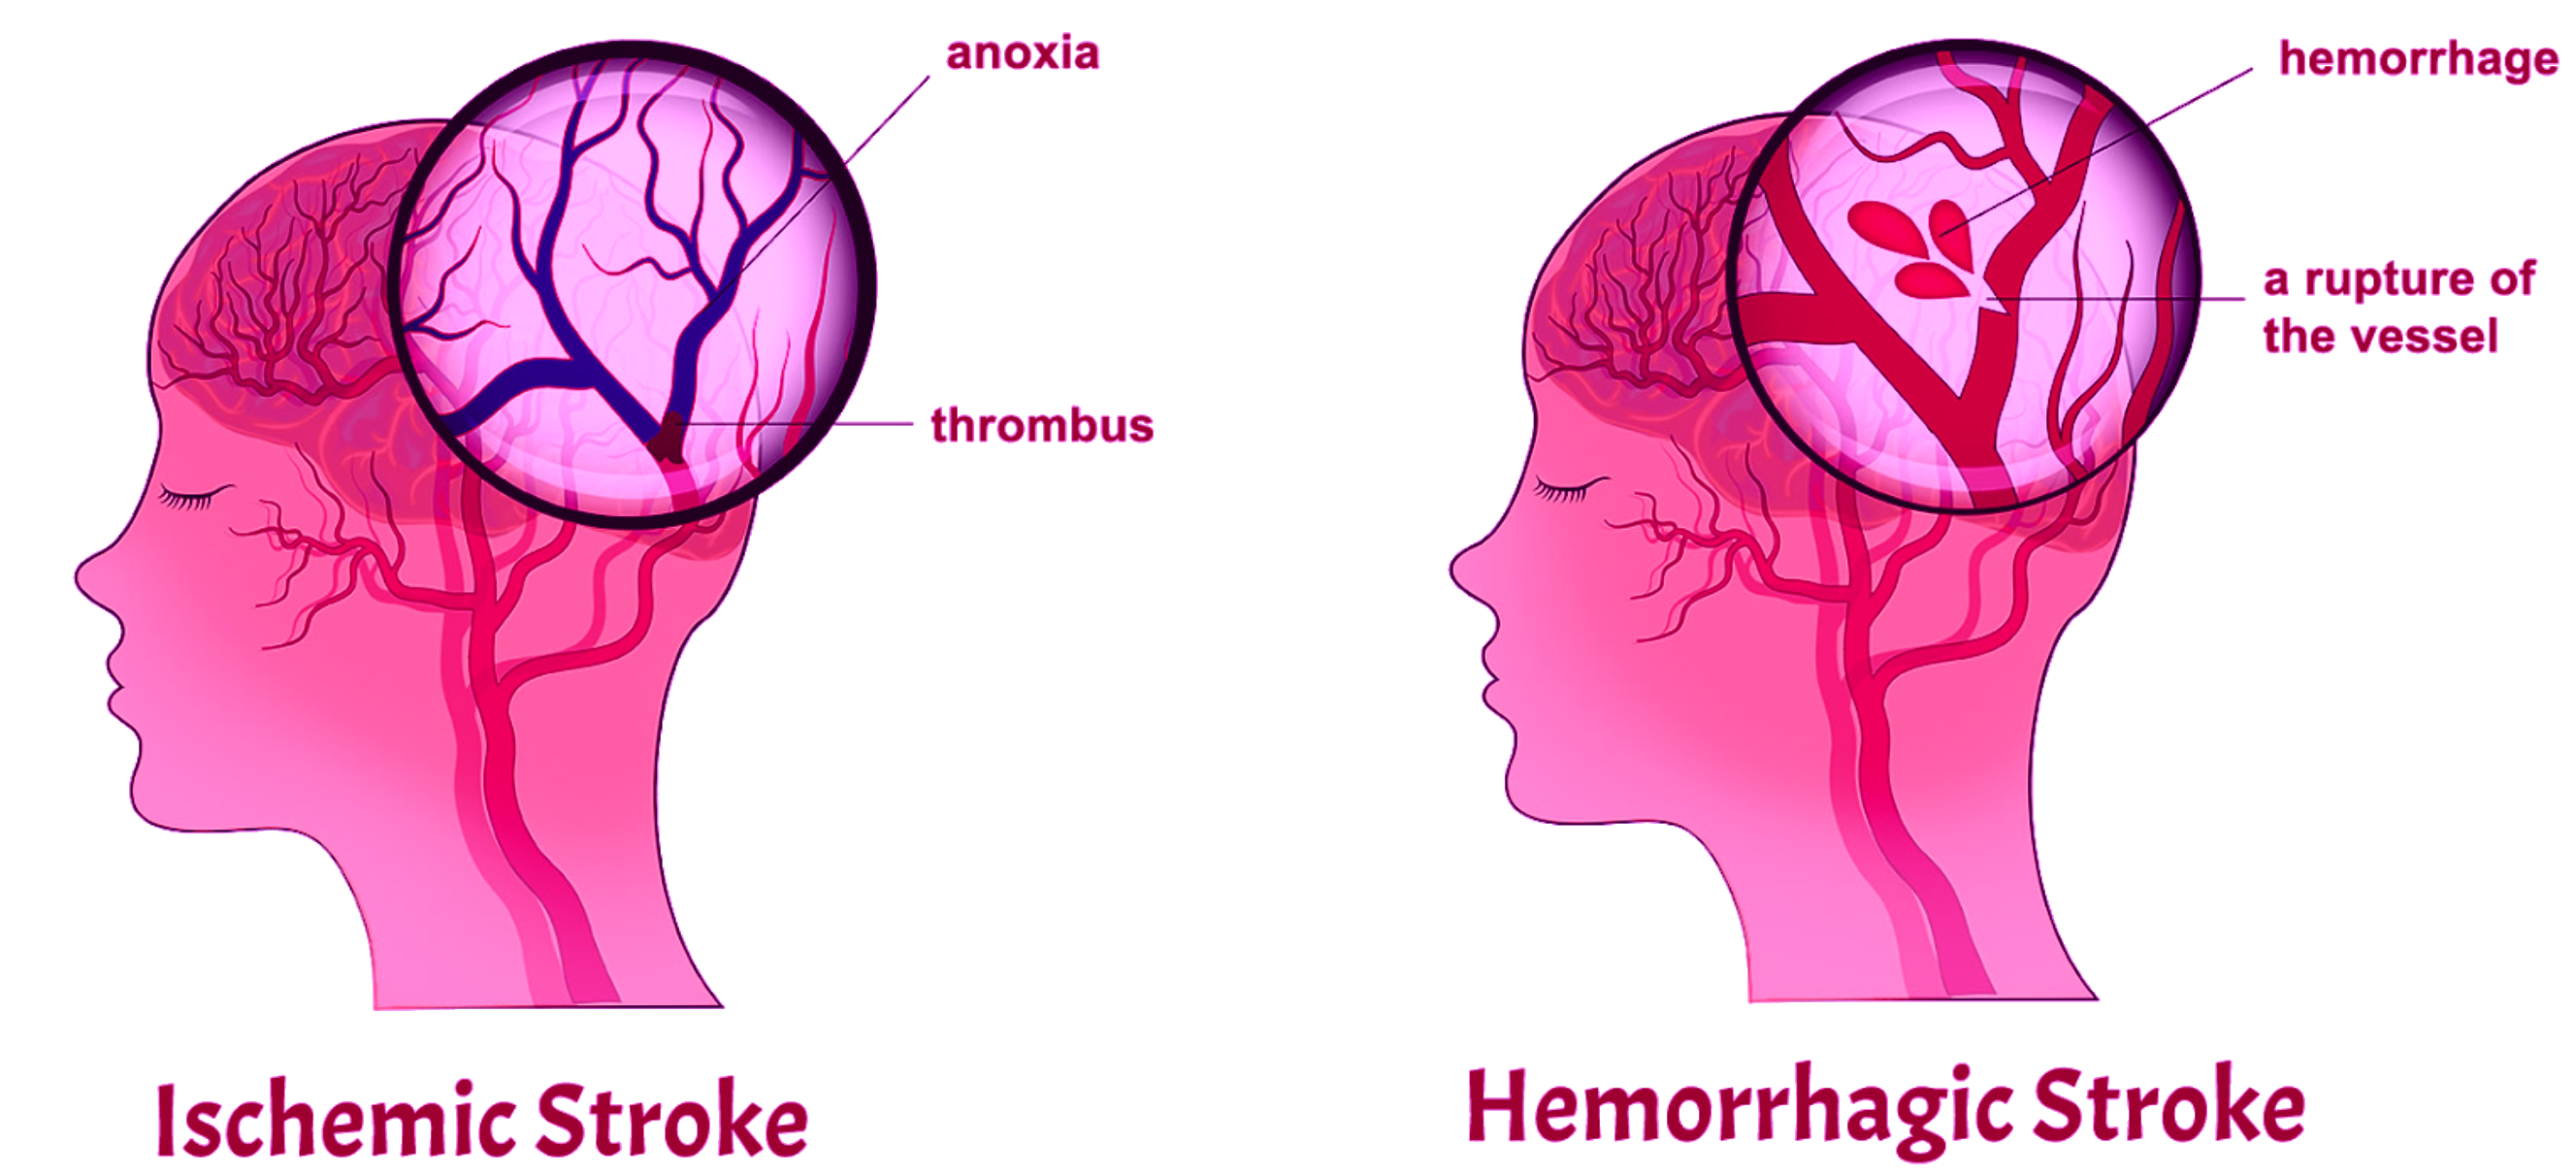
\includegraphics[width=1.0\textwidth]{./images/stroke_types}
\end{center}


\end{frame}
\begin{frame}
\frametitle{Thrombolysis (\emph{'Clot-busting'} medication) in stroke}

While the clot is still fresh, thrombolysis may be given to help break down the clot and restore blood flow.

\vspace{3mm}

\begin{center}
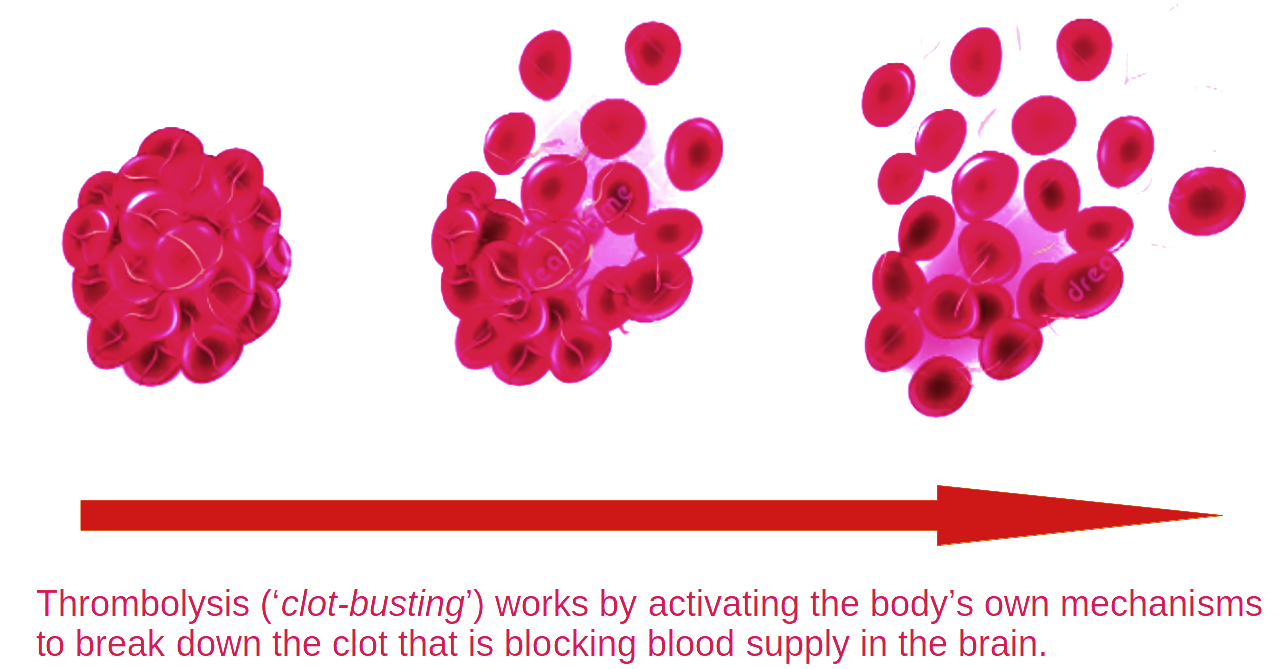
\includegraphics[width=0.70\textwidth]{./images/thrombolysis_mechanism}
\end{center}

\textbf{Drawbacks/limitations}: There is a risk of severe bleed (in about 1 in 50 patients on average, with risk increasing with stroke severity), and thrombolysis loses effectiveness over about the first 5-6 hours.

\end{frame}
\begin{frame}
\frametitle{Use of thrombolysis rates varies significantly between hospitals}

\small
Thrombolysis use varied from below 5\% to 25\% across the 132 acute stroke centres in England and Wales, 2016-2018.
\begin{center}
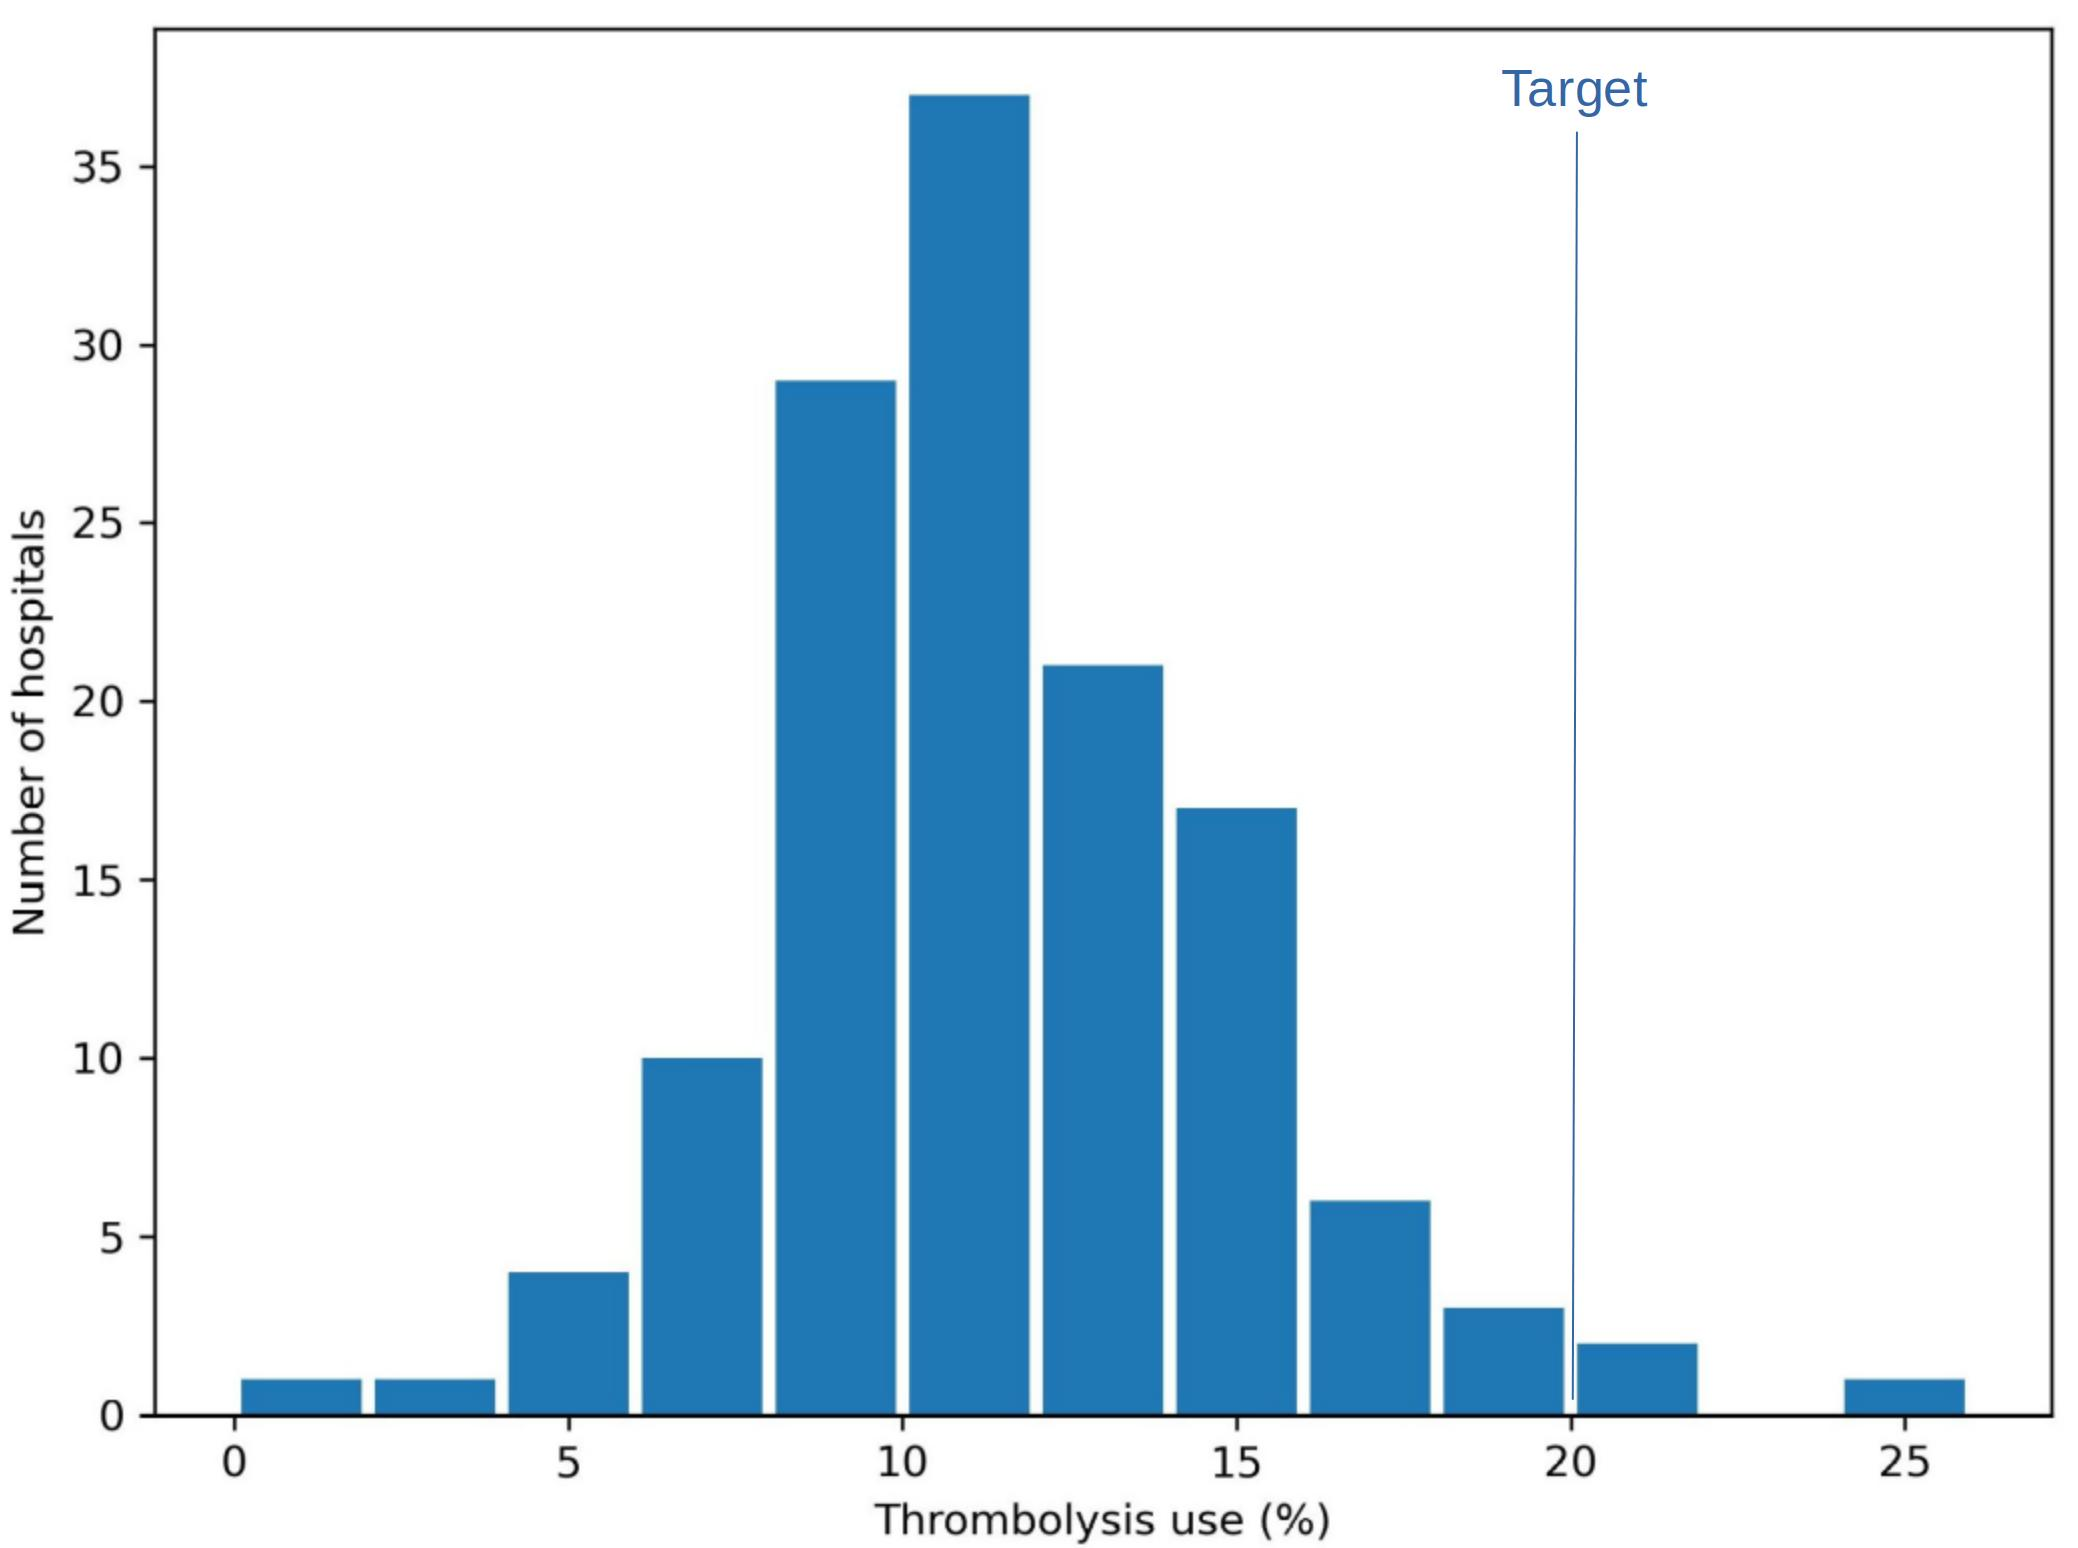
\includegraphics[width=0.50\textwidth]{./images/thrombolysis_by_hospital}
\end{center}

How much of this variation is due to differences in local patient populations, and how much is due to differences in in-hospital processes and decisions hospitals make on who they would give thrombolysis to?
\end{frame}
\begin{frame}
\frametitle{Thrombolysis pathway}
A simplified representation of the thrombolysis pathway as we model it.
\vspace{10mm}
\begin{center}
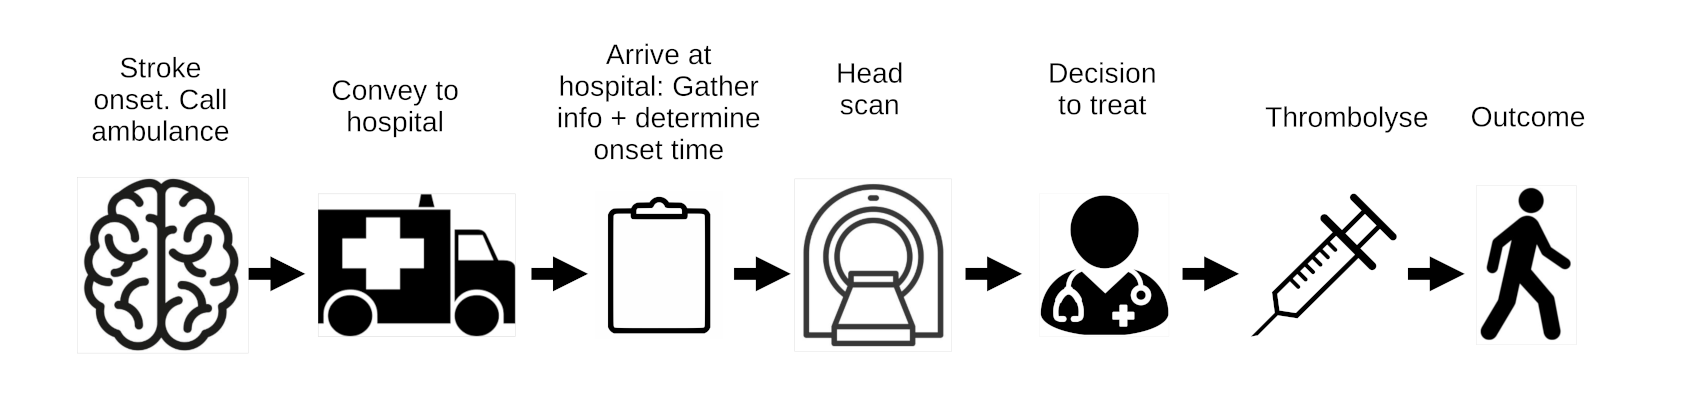
\includegraphics[width=1.0\textwidth]{./images/pathway}
\end{center}
\end{frame}
\begin{frame}
\frametitle{Machine learning overview}
\begin{center}
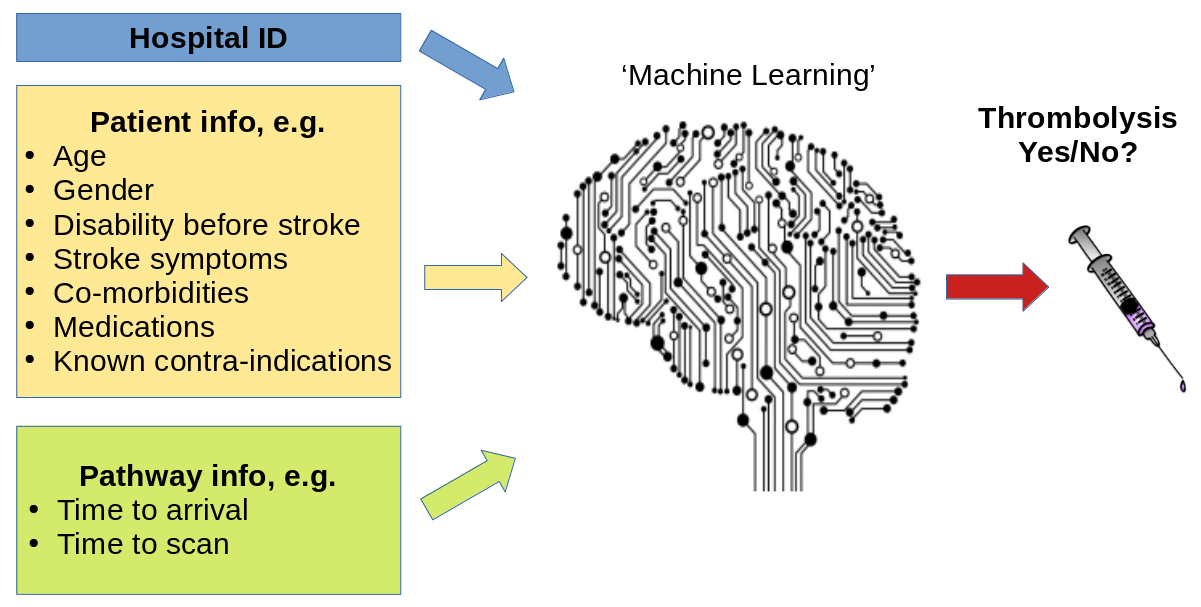
\includegraphics[width=0.80\textwidth]{./images/ml_model_high_level}
\end{center}

\small
\textbf{Machine learning is based on the simple principle of recognising similarity to what has been seen before.}
\vspace{2mm}

\footnotesize{We accessed 246,676 emergency stroke admissions in England and Wales over three years. Our machine learning models use XGBoost classification, and are based on those 88,928 patients who arrive within 4 hours of known stroke onset. Accuracy = 85\% (ROC AUC = 0.92).}
\end{frame}
\begin{frame}{Model accuracy, and simplification}

A model with all available 84 features had an ROC AUC of 0.922. A model with 10 features had an ROC AUC of 0.919.

\begin{center}
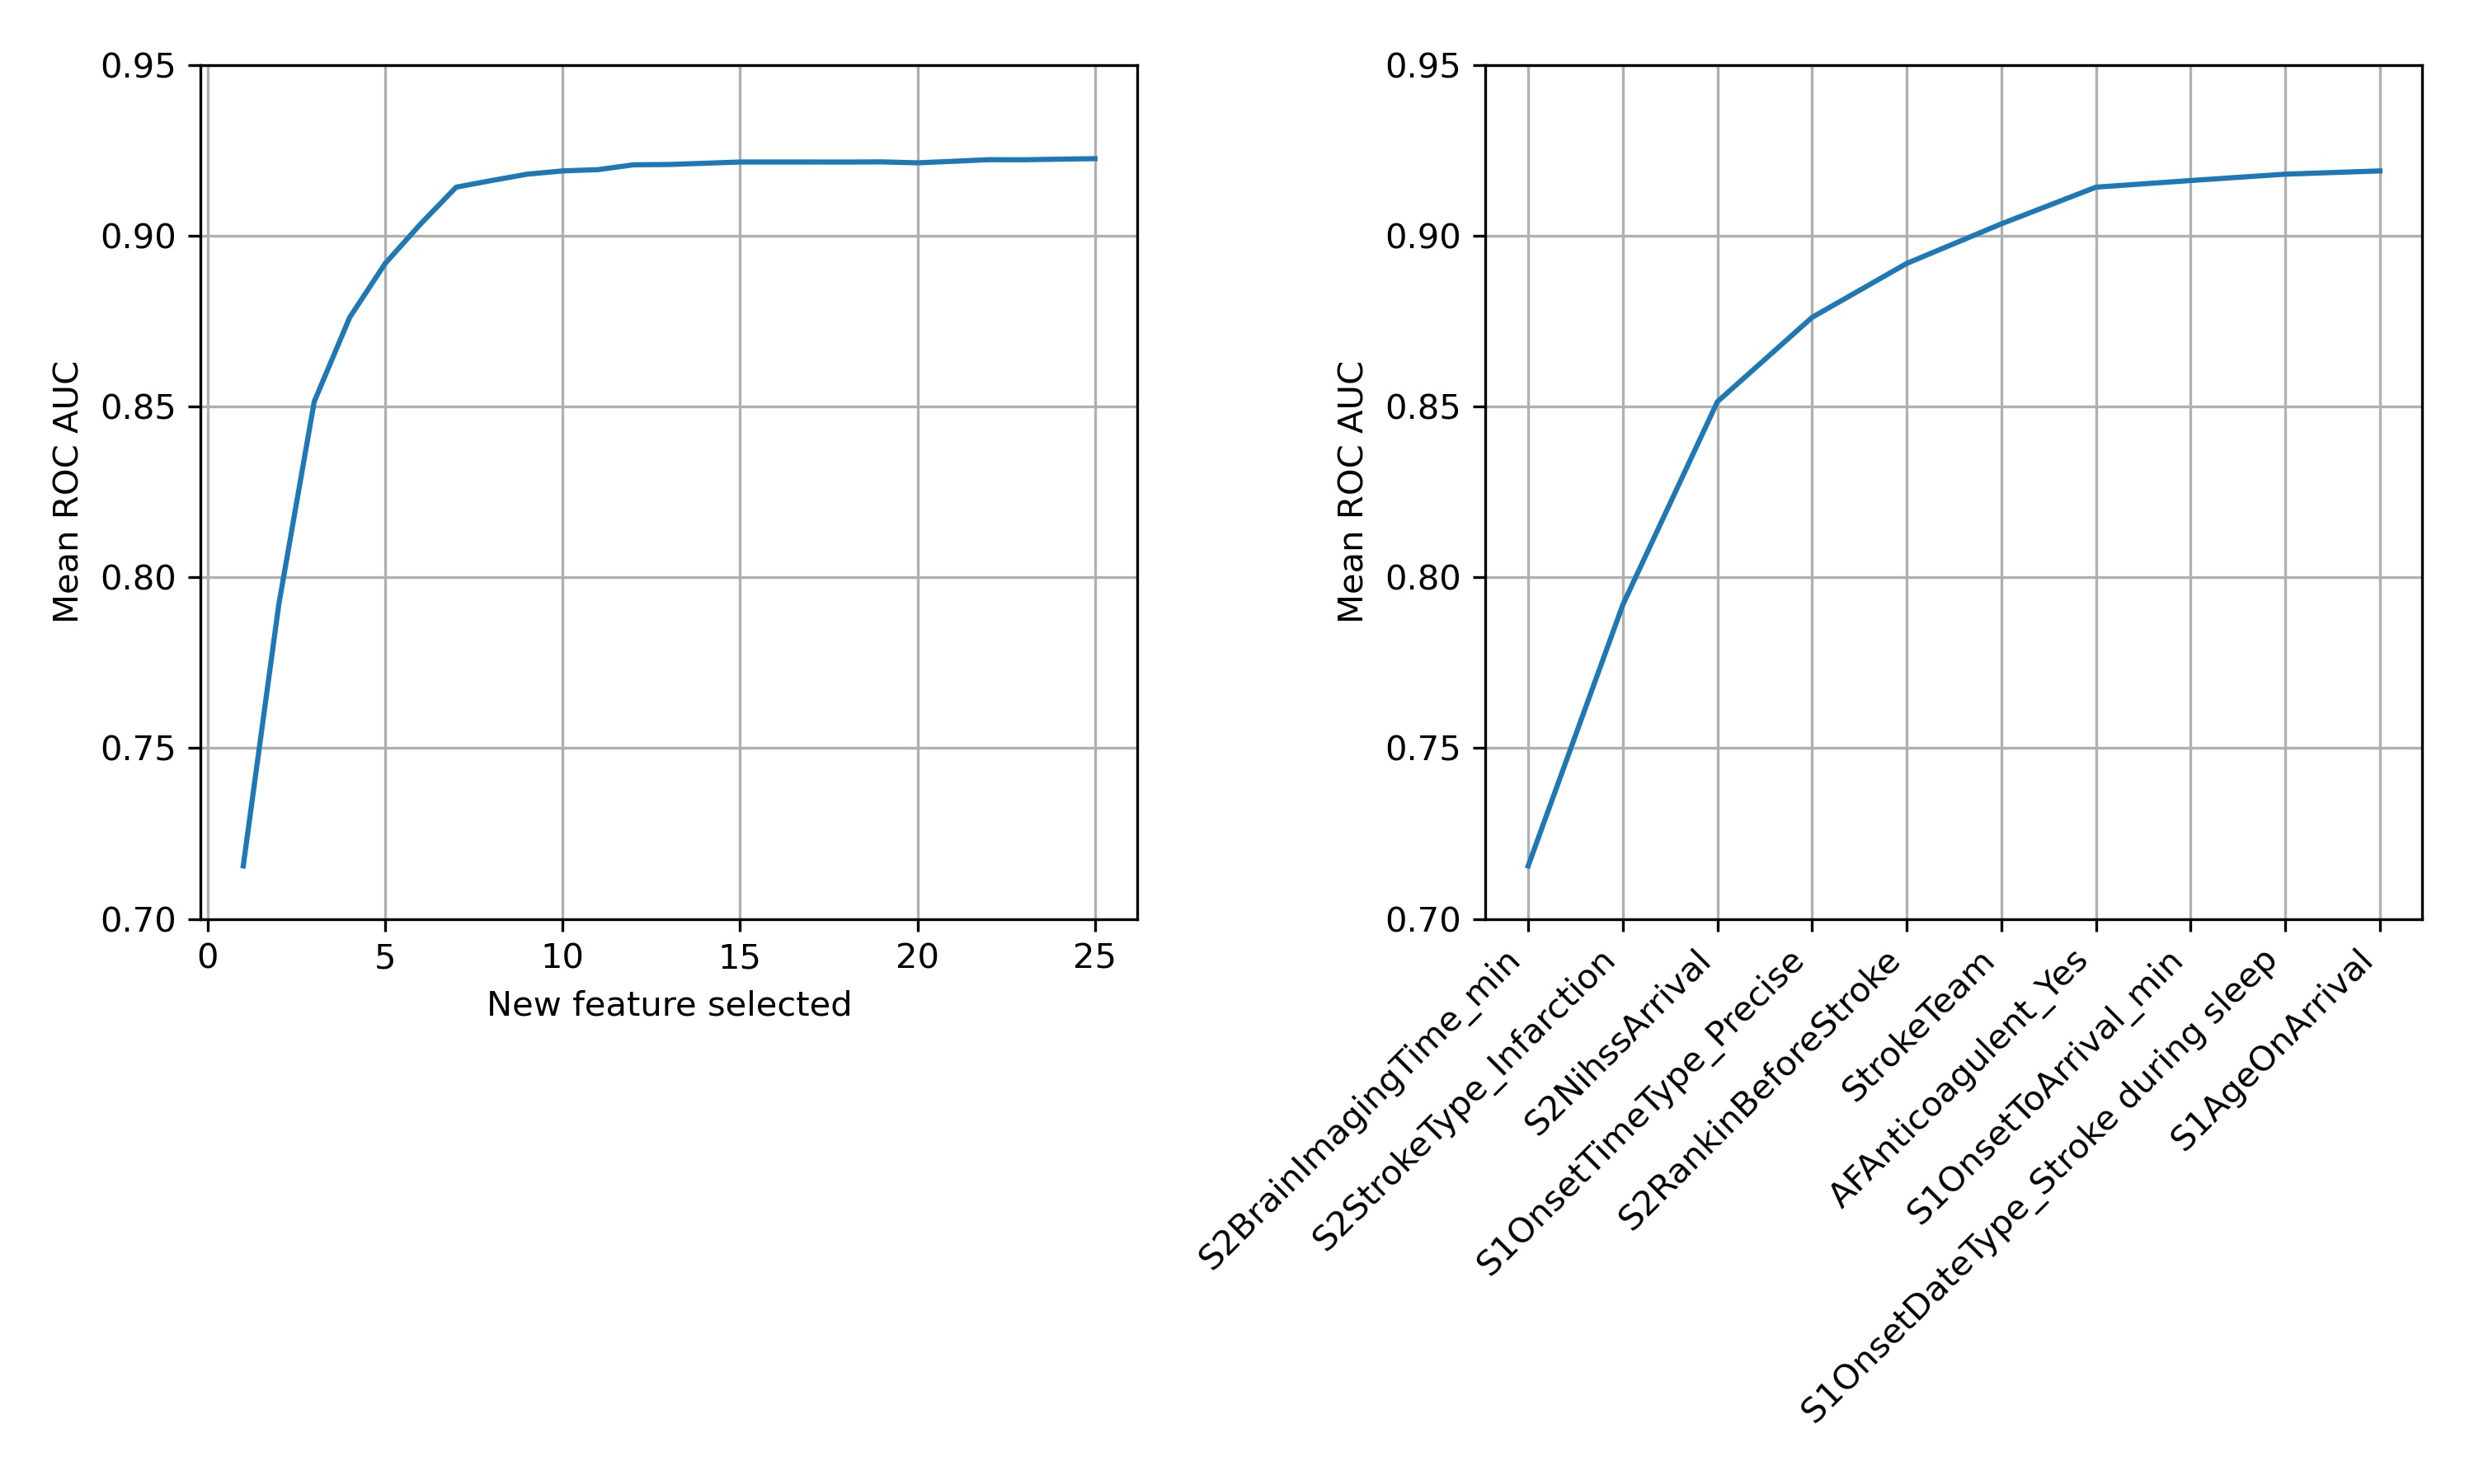
\includegraphics[width=0.9\textwidth]{./images/01_feature_selection.jpg}
\end{center}

Our simpler machine learning model will just use these 10 features.

\end{frame}
\begin{frame}{Predicting hospital thrombolysis use}

Predicted thrombolysis use was measured by combining 5 test sets from k-fold validation. The predicted vs. observed thrombolysis are highly correlated (r-squared 0.977). 

\begin{center}
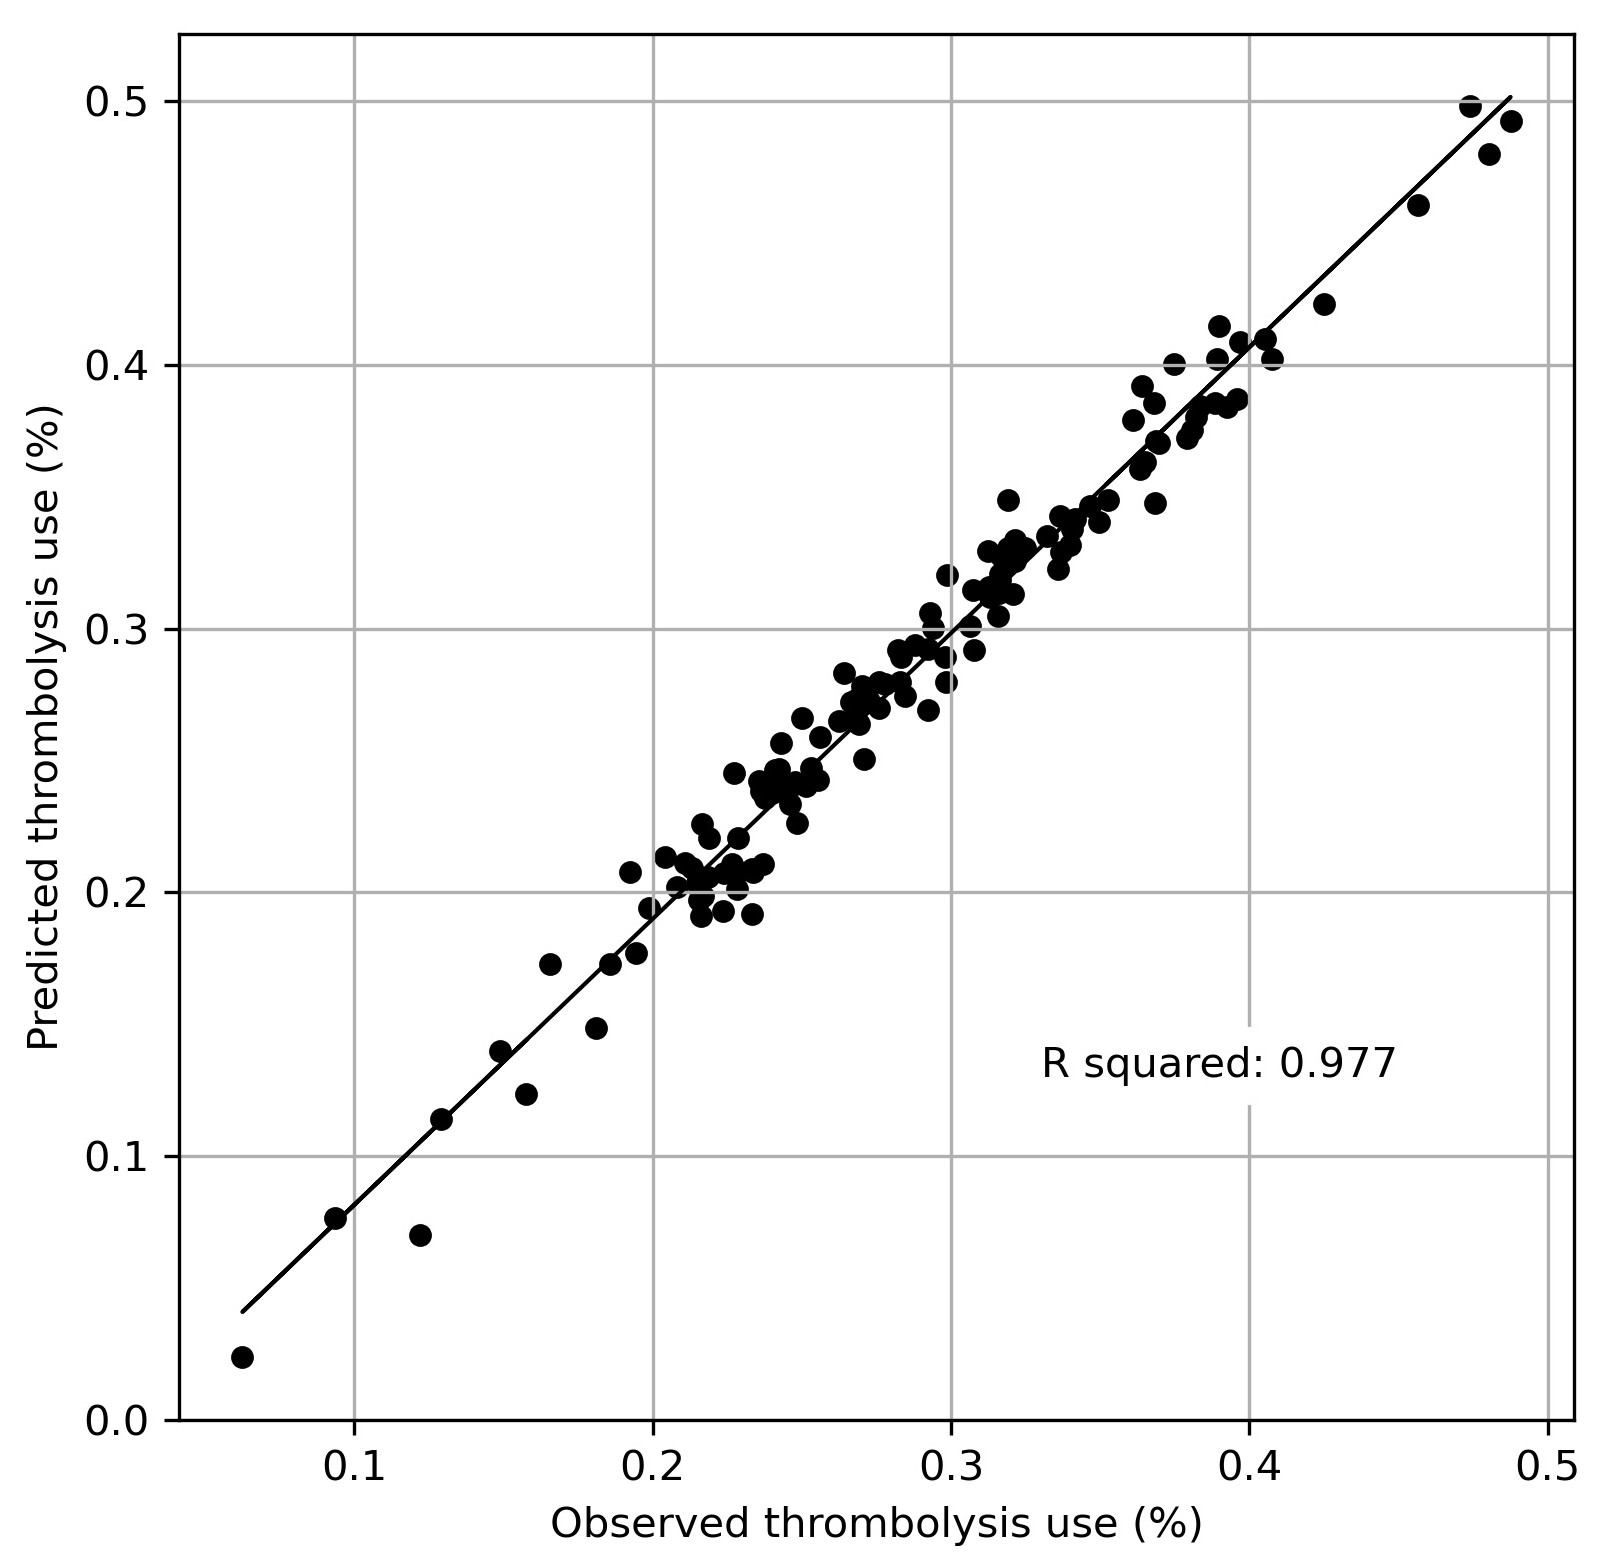
\includegraphics[width=0.55\textwidth]{./images/02_xgb_10_features_observed_predicted_rates.jpg}
\end{center}



\end{frame}
\begin{frame}
\frametitle{Explaining model predictions with SHAP values}

SHAP values show the influence of features (even for \emph{`black box'} models).

\begin{center}
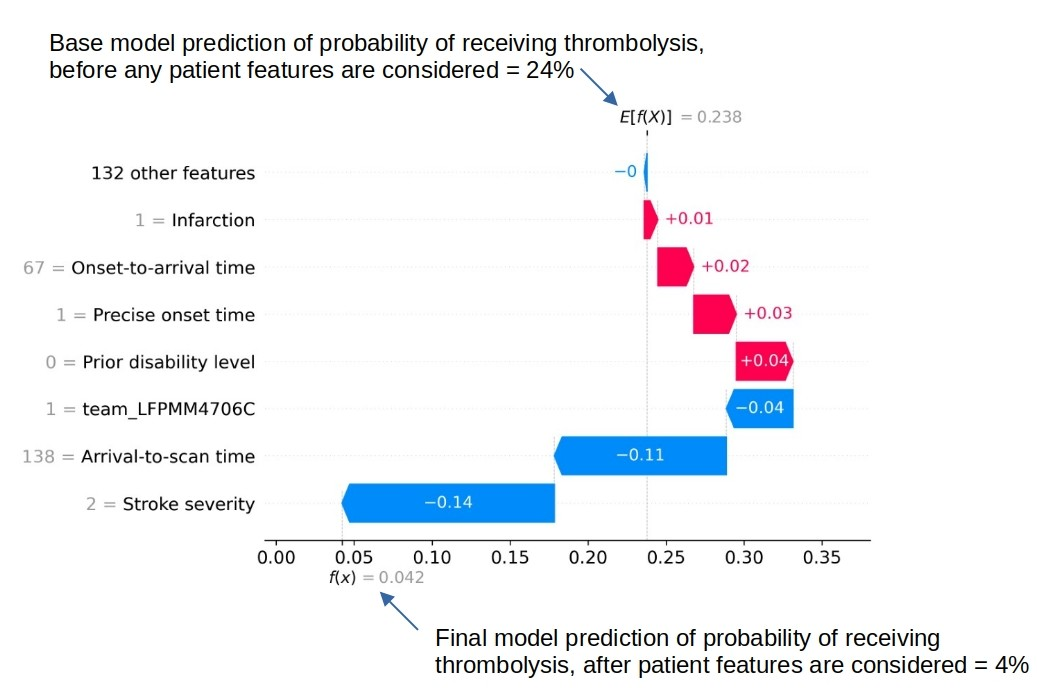
\includegraphics[width=0.90\textwidth]{./images/xgb_waterfall_low_probability_2.jpg}
\end{center}
\end{frame}
\begin{frame}
\frametitle{SHAP values for thrombolysis prediction}
Note: SHAP values here are log odds. 
\begin{center}
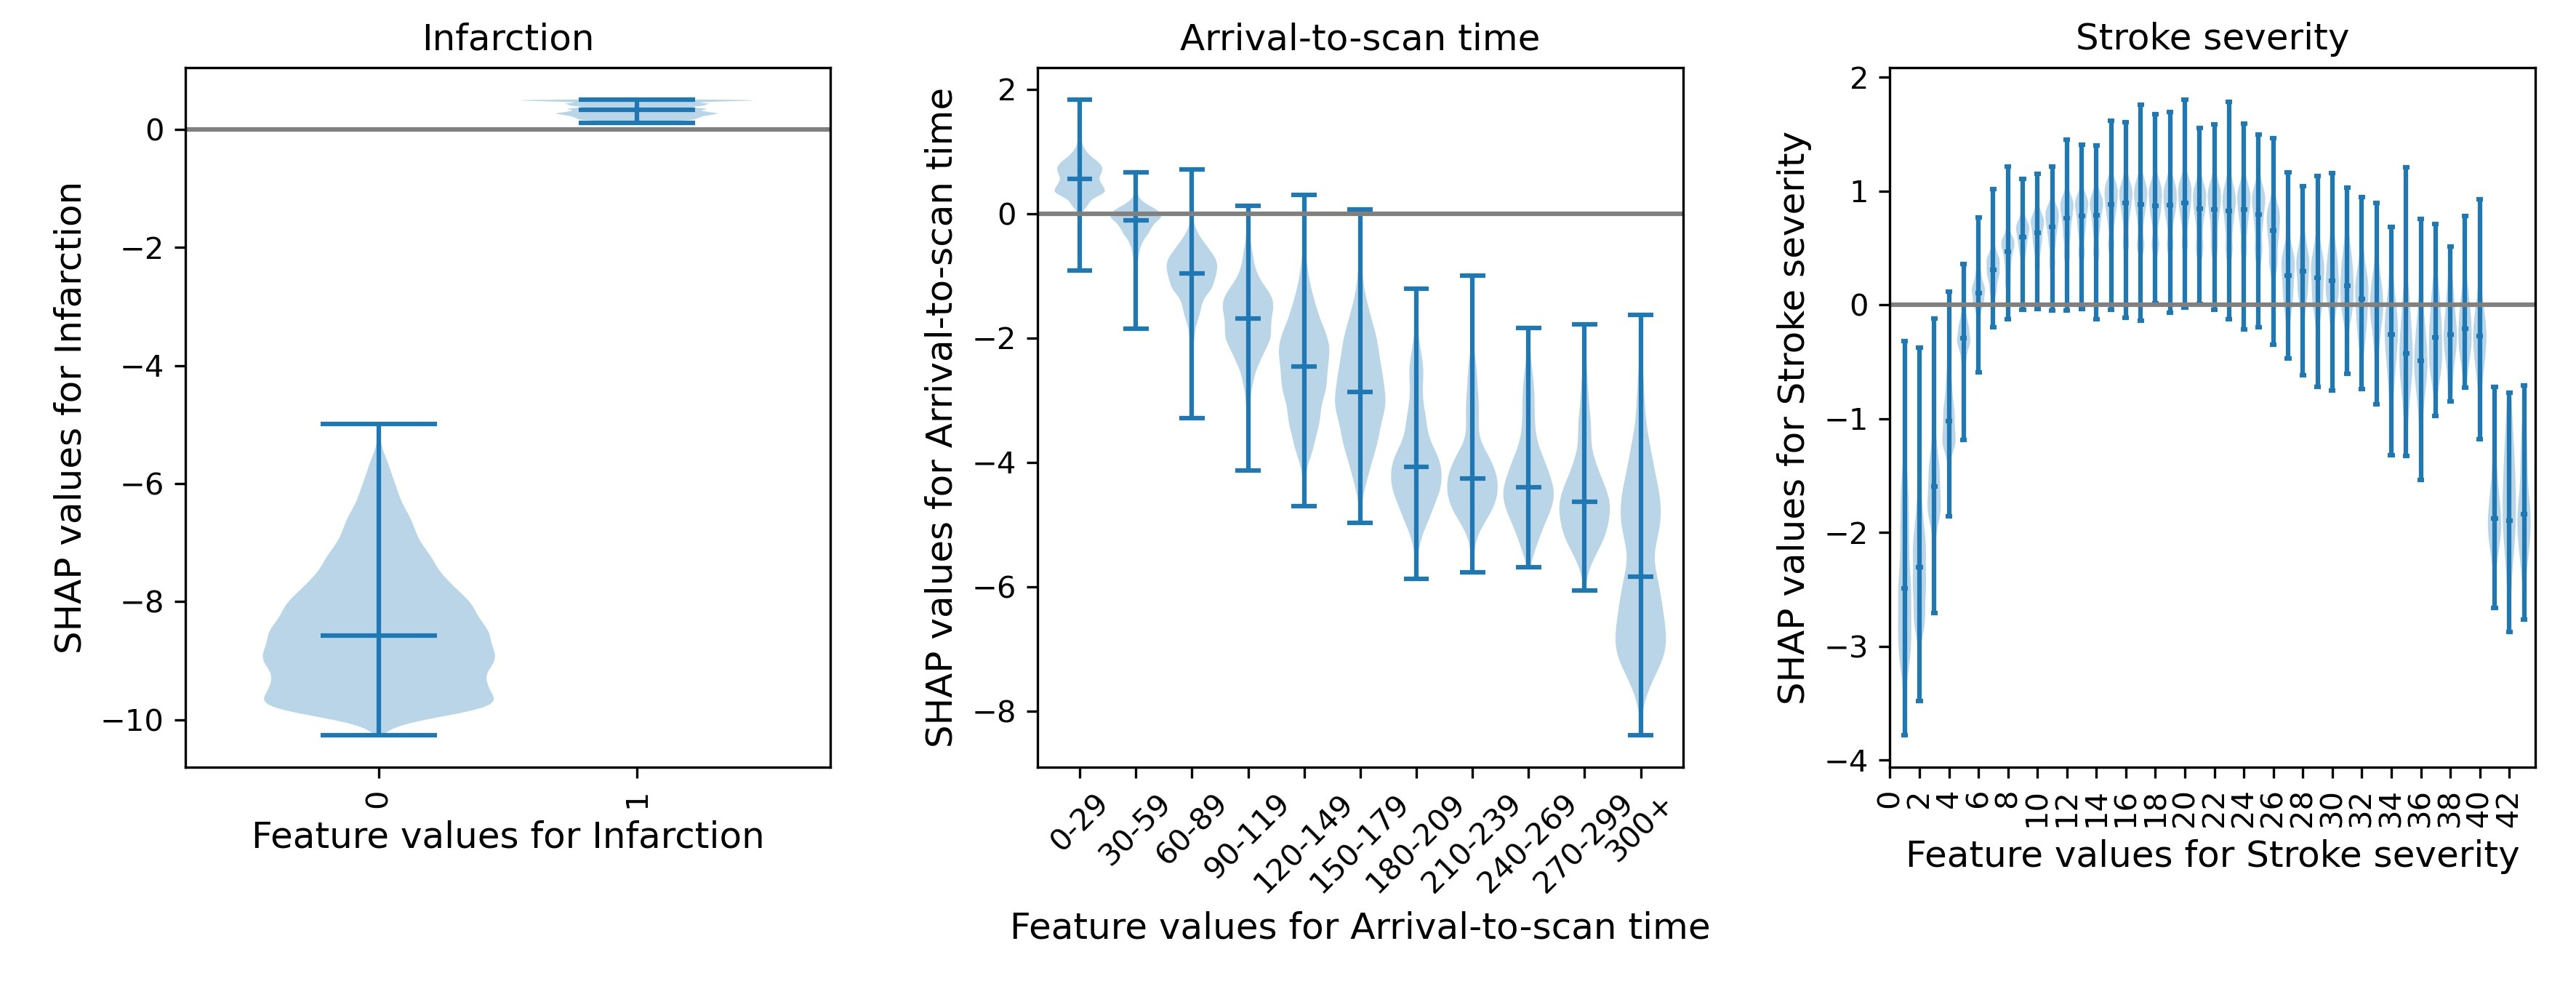
\includegraphics[width=1.0\textwidth]{./images/03d_xgb_10_features_thrombolysis_shap_violin_1.jpg}
\end{center}

\scriptsize
SHAP effects: \\
$\pm1$: Odds change $\pm3$ fold\\
$\pm2$: Odds change $\pm7$ fold\\
$\pm3$: Odds change $\pm20$ fold\\
$\pm4$: Odds change $\pm55$ fold\\
$\pm5$: Odds change $\pm150$ fold
\end{frame}
\begin{frame}
\frametitle{SHAP values for each feature - 2}
Note: SHAP values here are log odds. 
\begin{center}
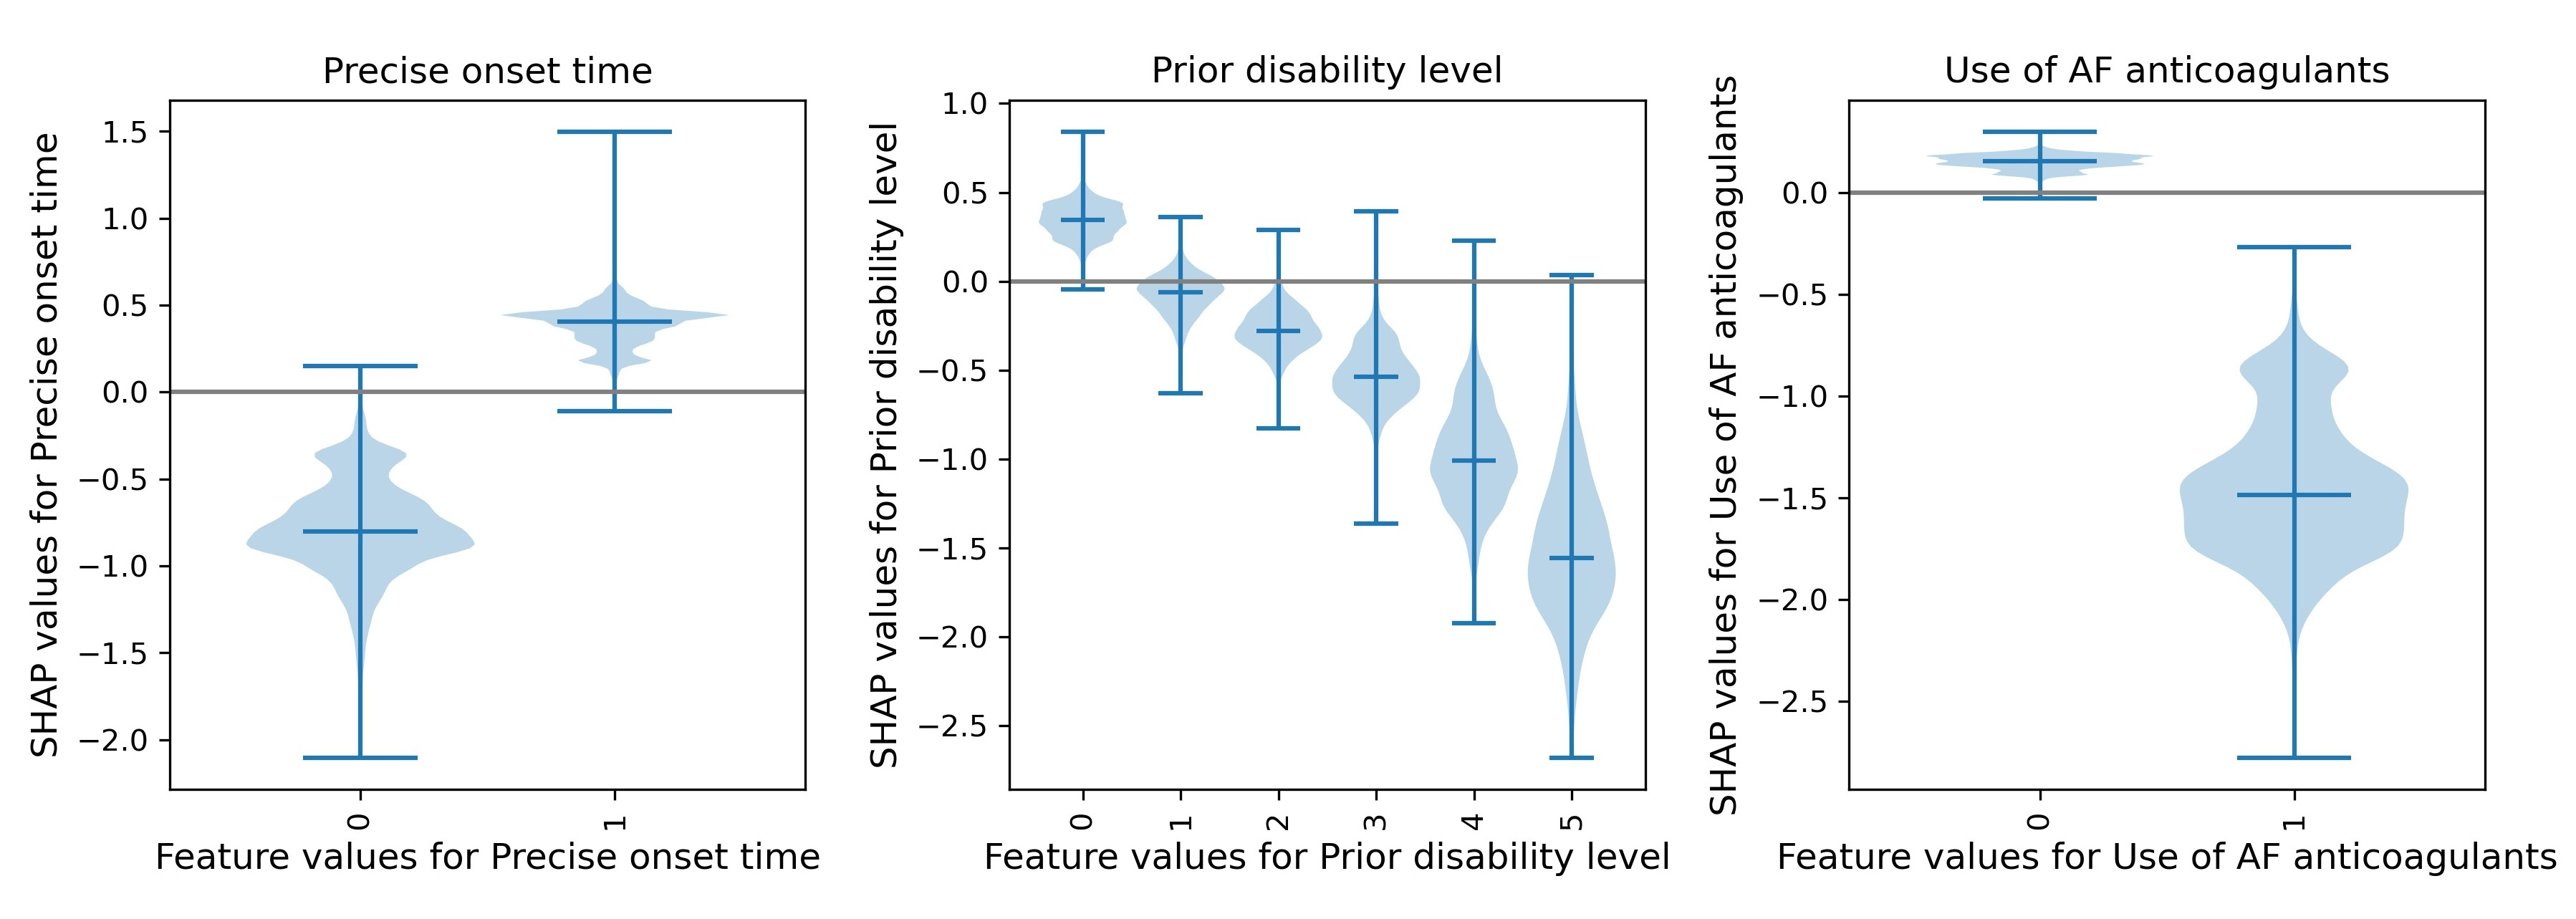
\includegraphics[width=1.0\textwidth]{./images/03d_xgb_10_features_thrombolysis_shap_violin_2.jpg}
\end{center}
\scriptsize
SHAP effects: \\
$\pm1$: Odds change $\pm3$ fold\\
$\pm2$: Odds change $\pm7$ fold\\
$\pm3$: Odds change $\pm20$ fold\\
$\pm4$: Odds change $\pm55$ fold\\
$\pm5$: Odds change $\pm150$ fold
\end{frame}
\begin{frame}
\frametitle{SHAP values for each feature - 3}
Note: SHAP values here are log odds. 
\begin{center}
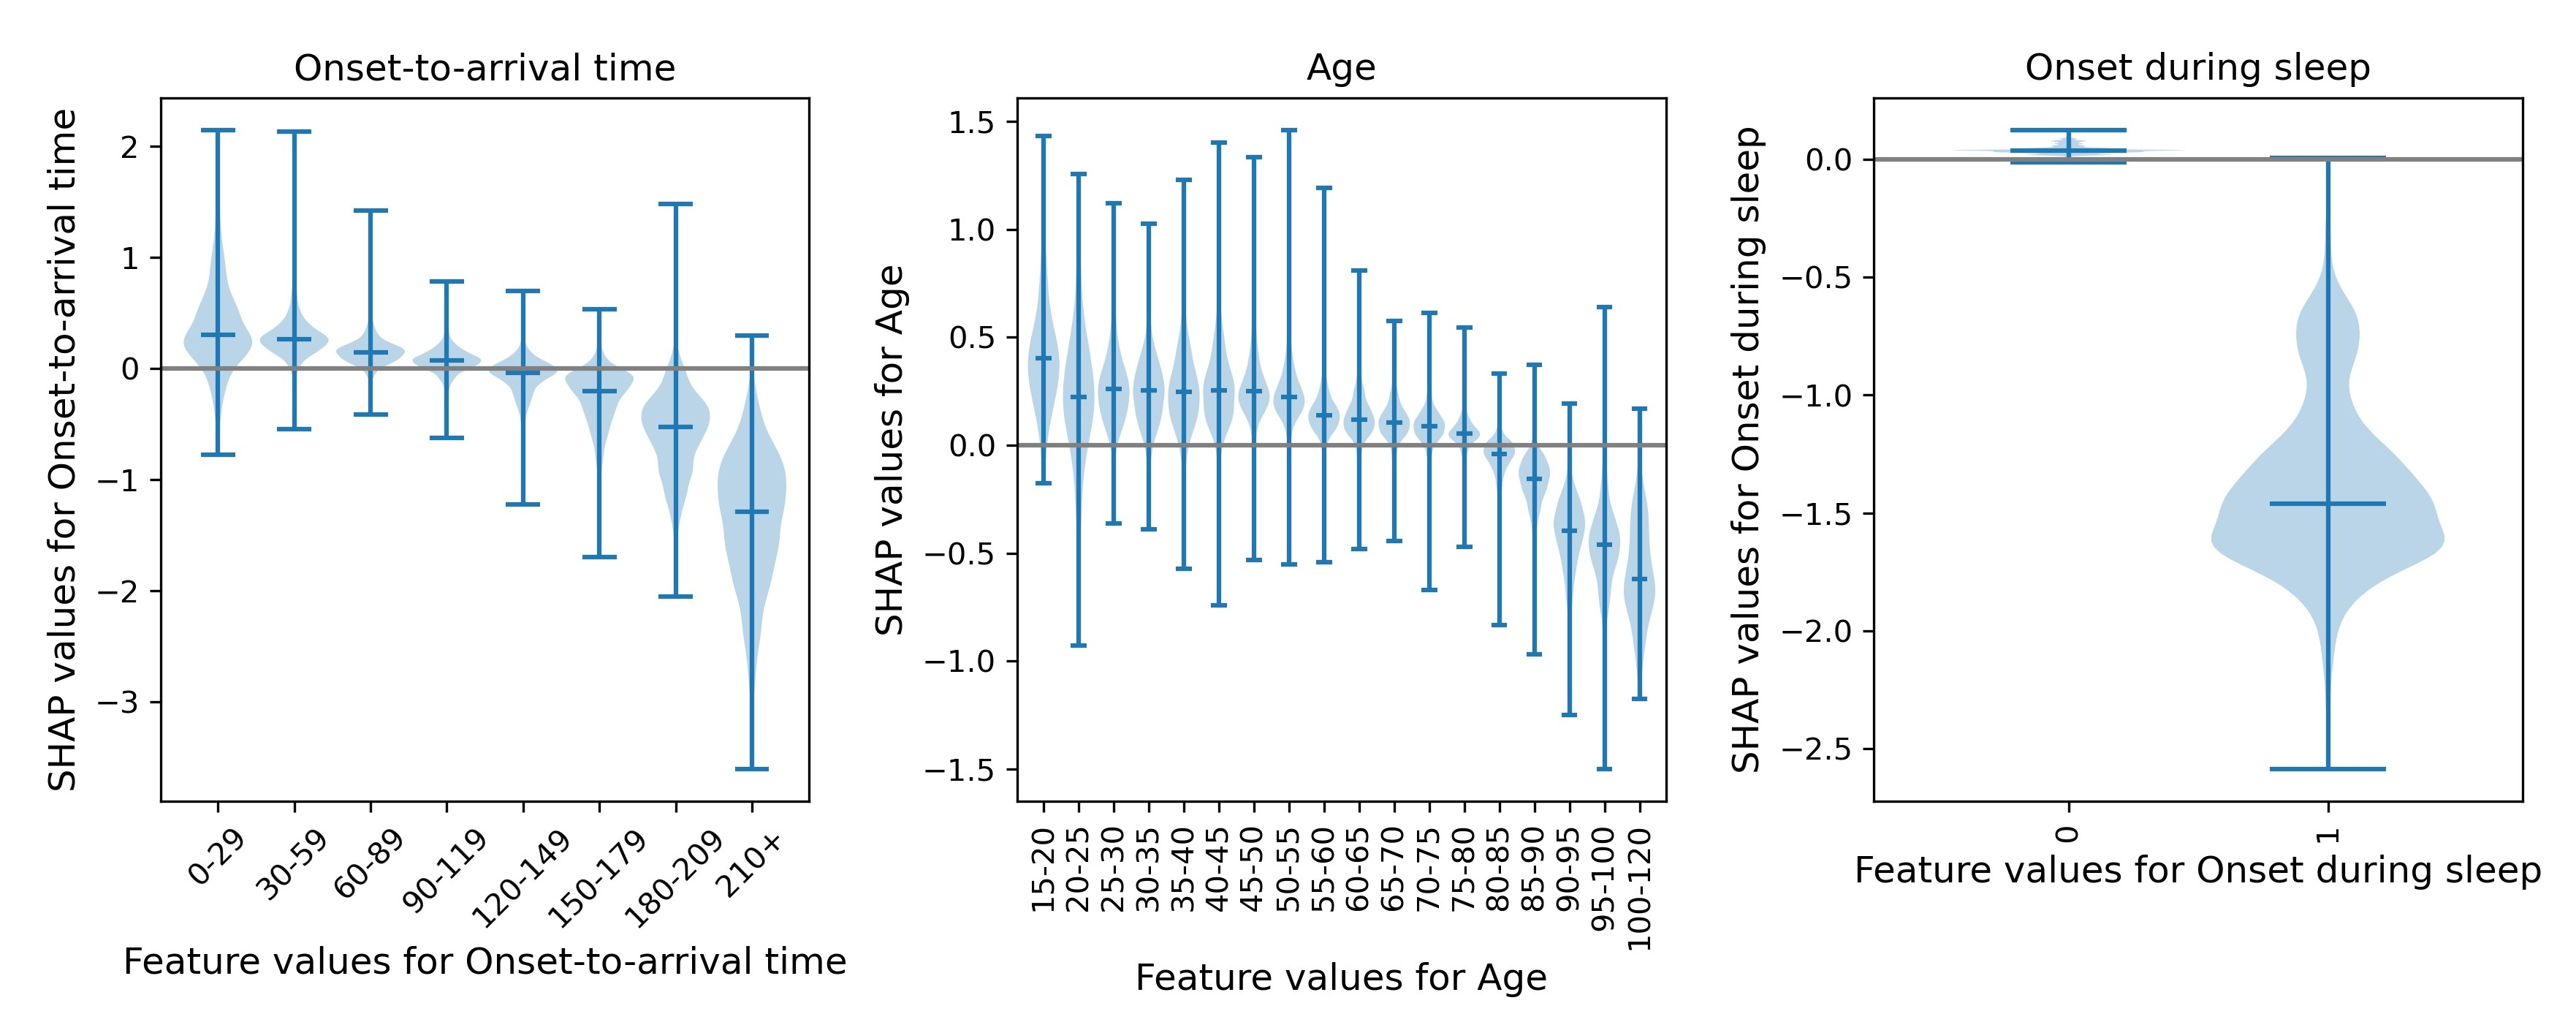
\includegraphics[width=1.0\textwidth]{./images/03d_xgb_10_features_thrombolysis_shap_violin_3.jpg}
\end{center}
\scriptsize
SHAP effects: \\
$\pm1$: Odds change $\pm3$ fold\\
$\pm2$: Odds change $\pm7$ fold\\
$\pm3$: Odds change $\pm20$ fold\\
$\pm4$: Odds change $\pm55$ fold\\
$\pm5$: Odds change $\pm150$ fold
\end{frame}
\begin{frame}
\frametitle{Isolating the effect of hospitals}
Note: SHAP values here are log odds. 
\begin{center}
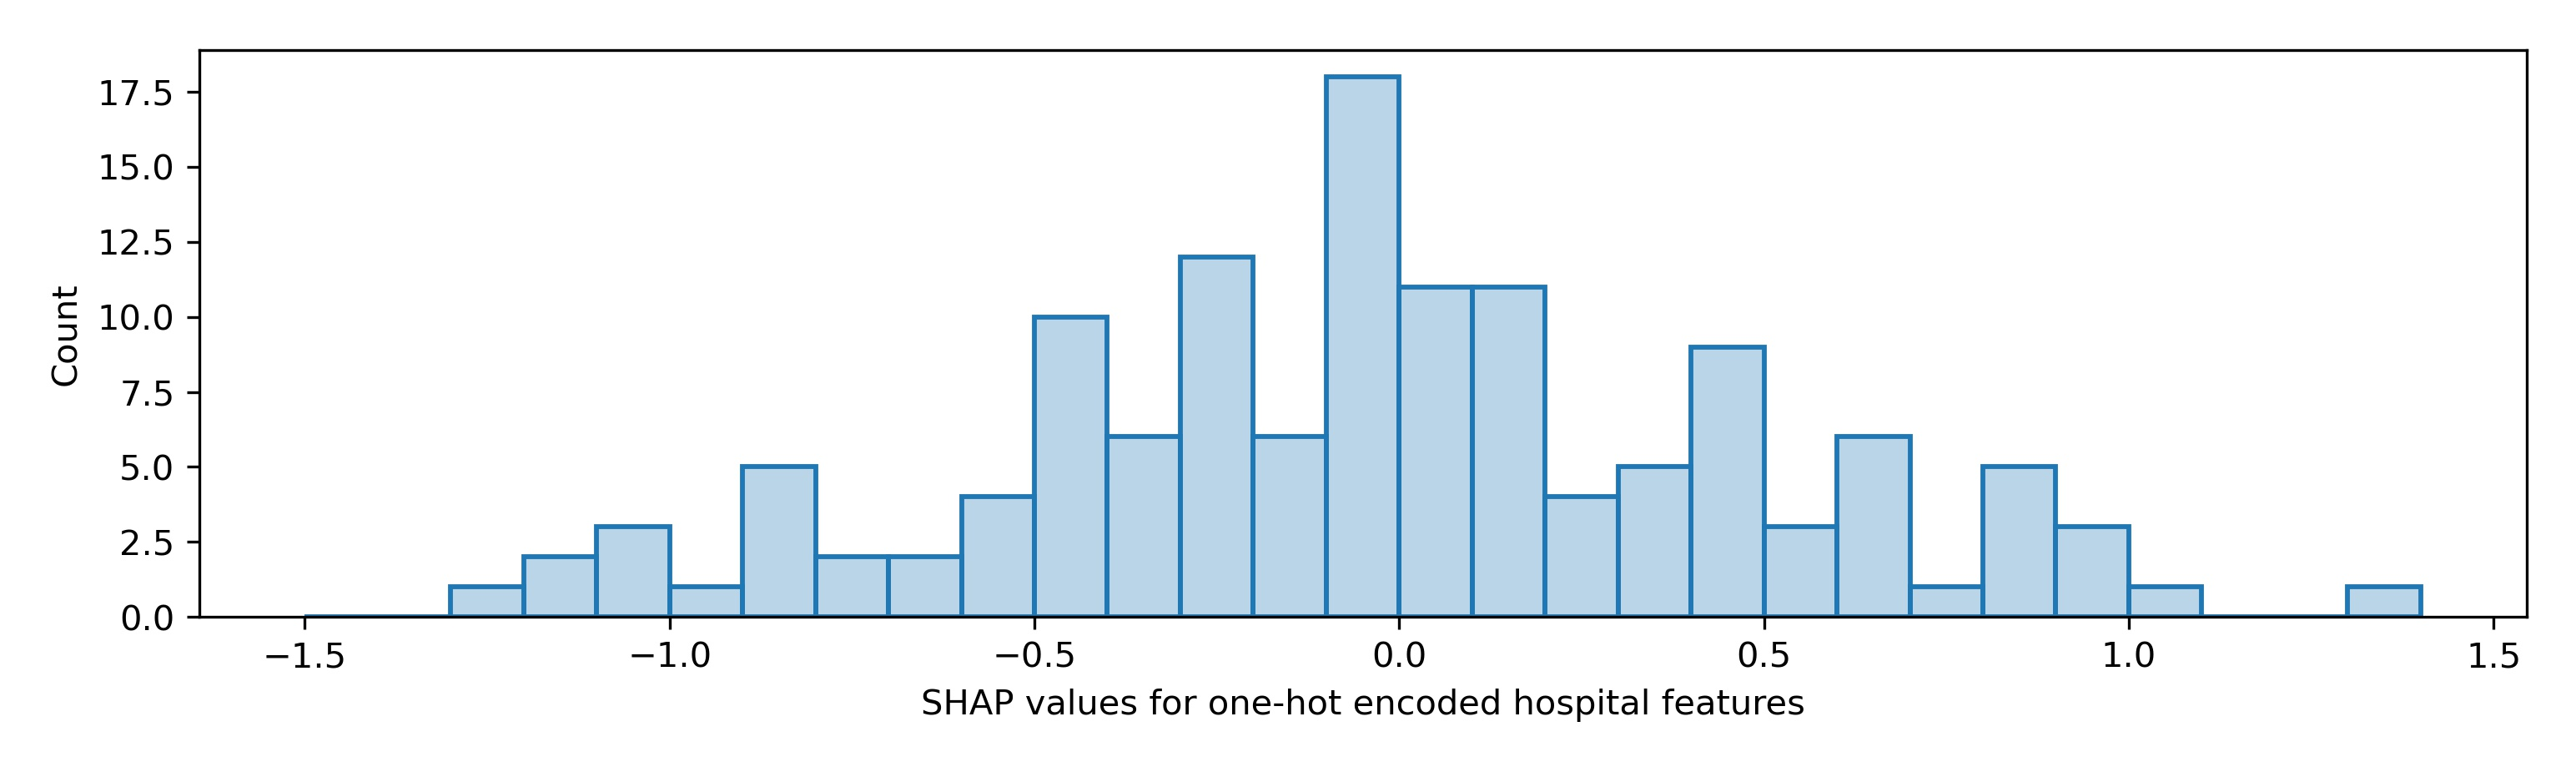
\includegraphics[width=1.0\textwidth]{./images/03d_xgb_10_features_hosp_shap_hist.jpg}
\end{center}
\scriptsize
SHAP effects: \\
$\pm1$: Odds change $\pm3$ fold\\
$\pm2$: Odds change $\pm7$ fold\\
$\pm3$: Odds change $\pm20$ fold\\
$\pm4$: Odds change $\pm55$ fold\\
$\pm5$: Odds change $\pm150$ fold
\end{frame}
\begin{frame}
\frametitle{Hospital SHAP predicts a hospital's predisposition to use thrombolysis}

\footnotesize Here we show the relationship of hospital SHAP with the hospital thrombolysis use for 1) the hospitals own patients, and 2) a common 10k cohort of patients.

\begin{center}
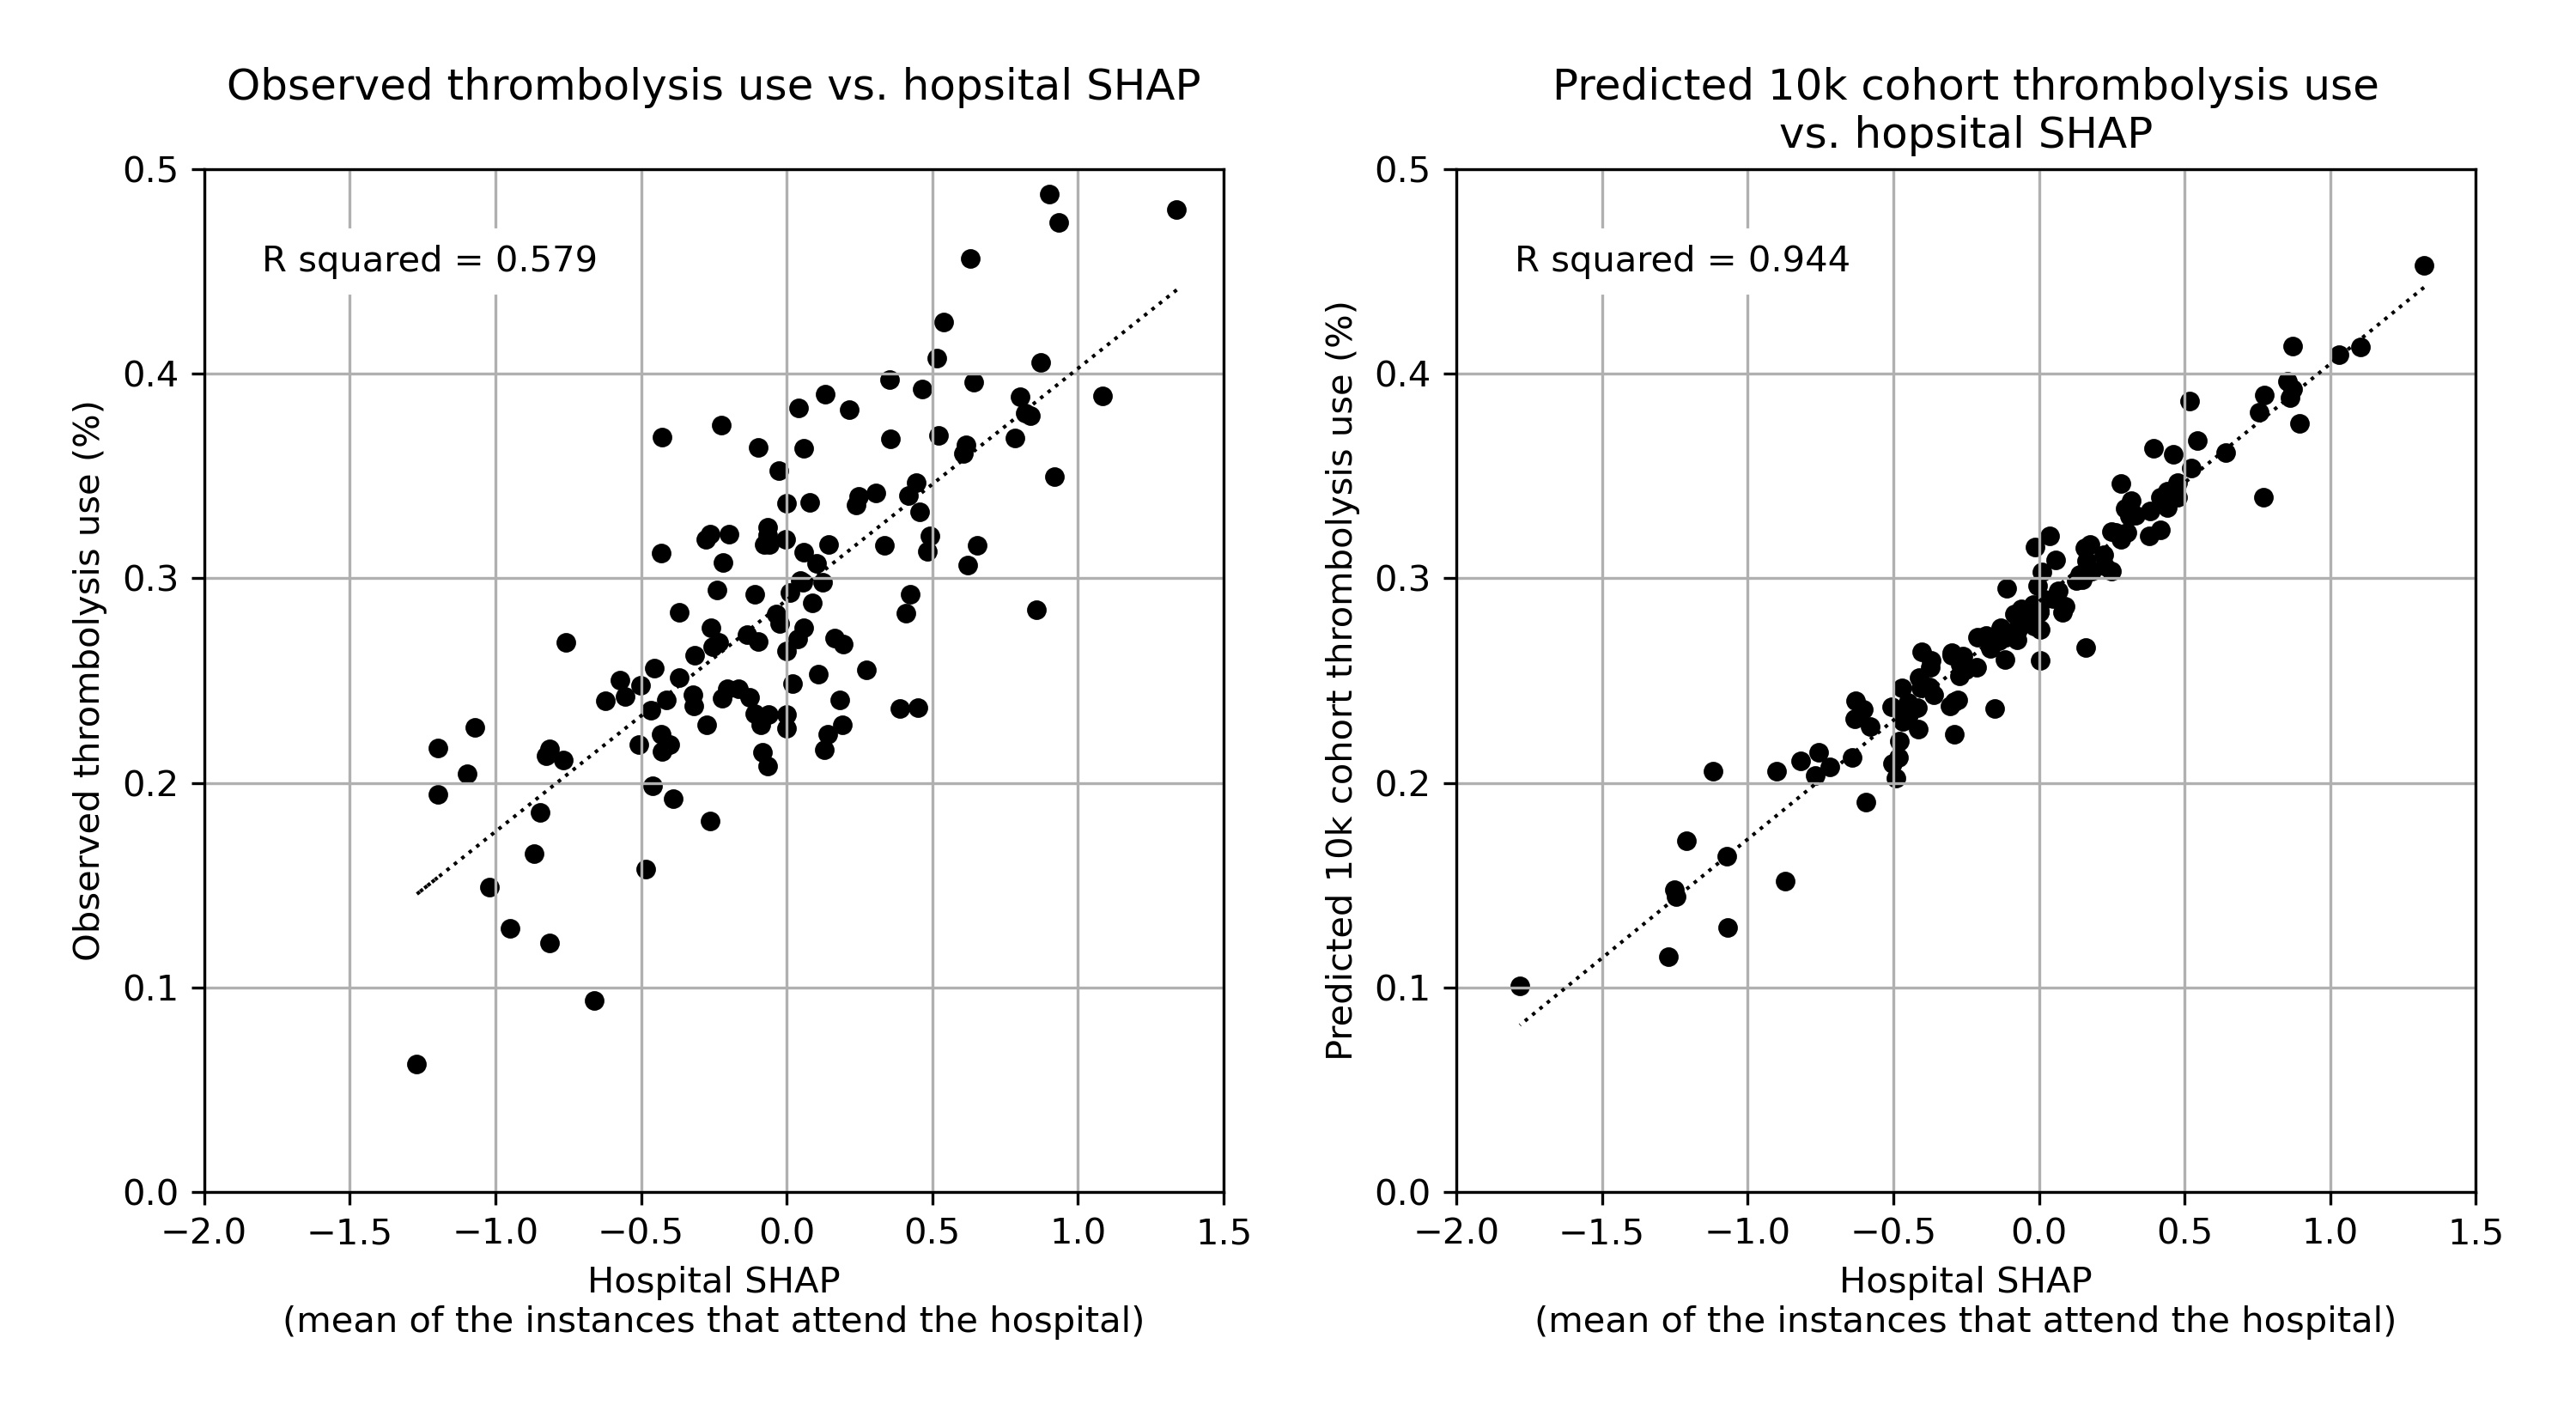
\includegraphics[width=1.0\textwidth]{./images/99_twin_correlation_scatter.jpg}
\end{center}
\end{frame}
\begin{frame}
\frametitle{We can predict what decision each hospital would make on different patients}

\vspace{3mm}

\begin{columns}[t]
    \begin{column}{0.45\textwidth}
        Base patient:
        \begin{itemize}
            \footnotesize
            \item Onset to arrival = 80 mins
            \item Arrival to scan = 20 mins
            \item Infarction = Yes
            \item NIHSS = 15
            \item Prior disability level = 0
            \item Precise onset time = Yes
            \item Use of AF anticoagulents = No
        \end{itemize}
    \end{column}
    
    \begin{column}{0.5\textwidth}
    \color{teal}
    Proportion of hospitals predicted to give thrombolysis:
    \footnotesize
    \begin{itemize}
        \color{teal}
        \item Base patient: 99\%
    \end{itemize}
    %\pause{} %Creates 2 PDF slides with pause here
    \vspace{3mm}
    \normalfont
    \color{red}
    \normalsize
    Base patient with:
    \footnotesize
    \begin{itemize}
        \color{red}
        \item NIHSS = 4: 73\%
        \item Pre-stroke mRS = 3: 86\%
        \item Estimated stroke onset time: 64\%
    \end{itemize}
    \end{column}

\end{columns}

\vspace{7mm}
This allows us to open up discussions between hospitals on differences in choices around thrombolysis.
\end{frame}

\begin{frame}
\frametitle{How would different teams respond to the same patient?}

    \begin{center}
    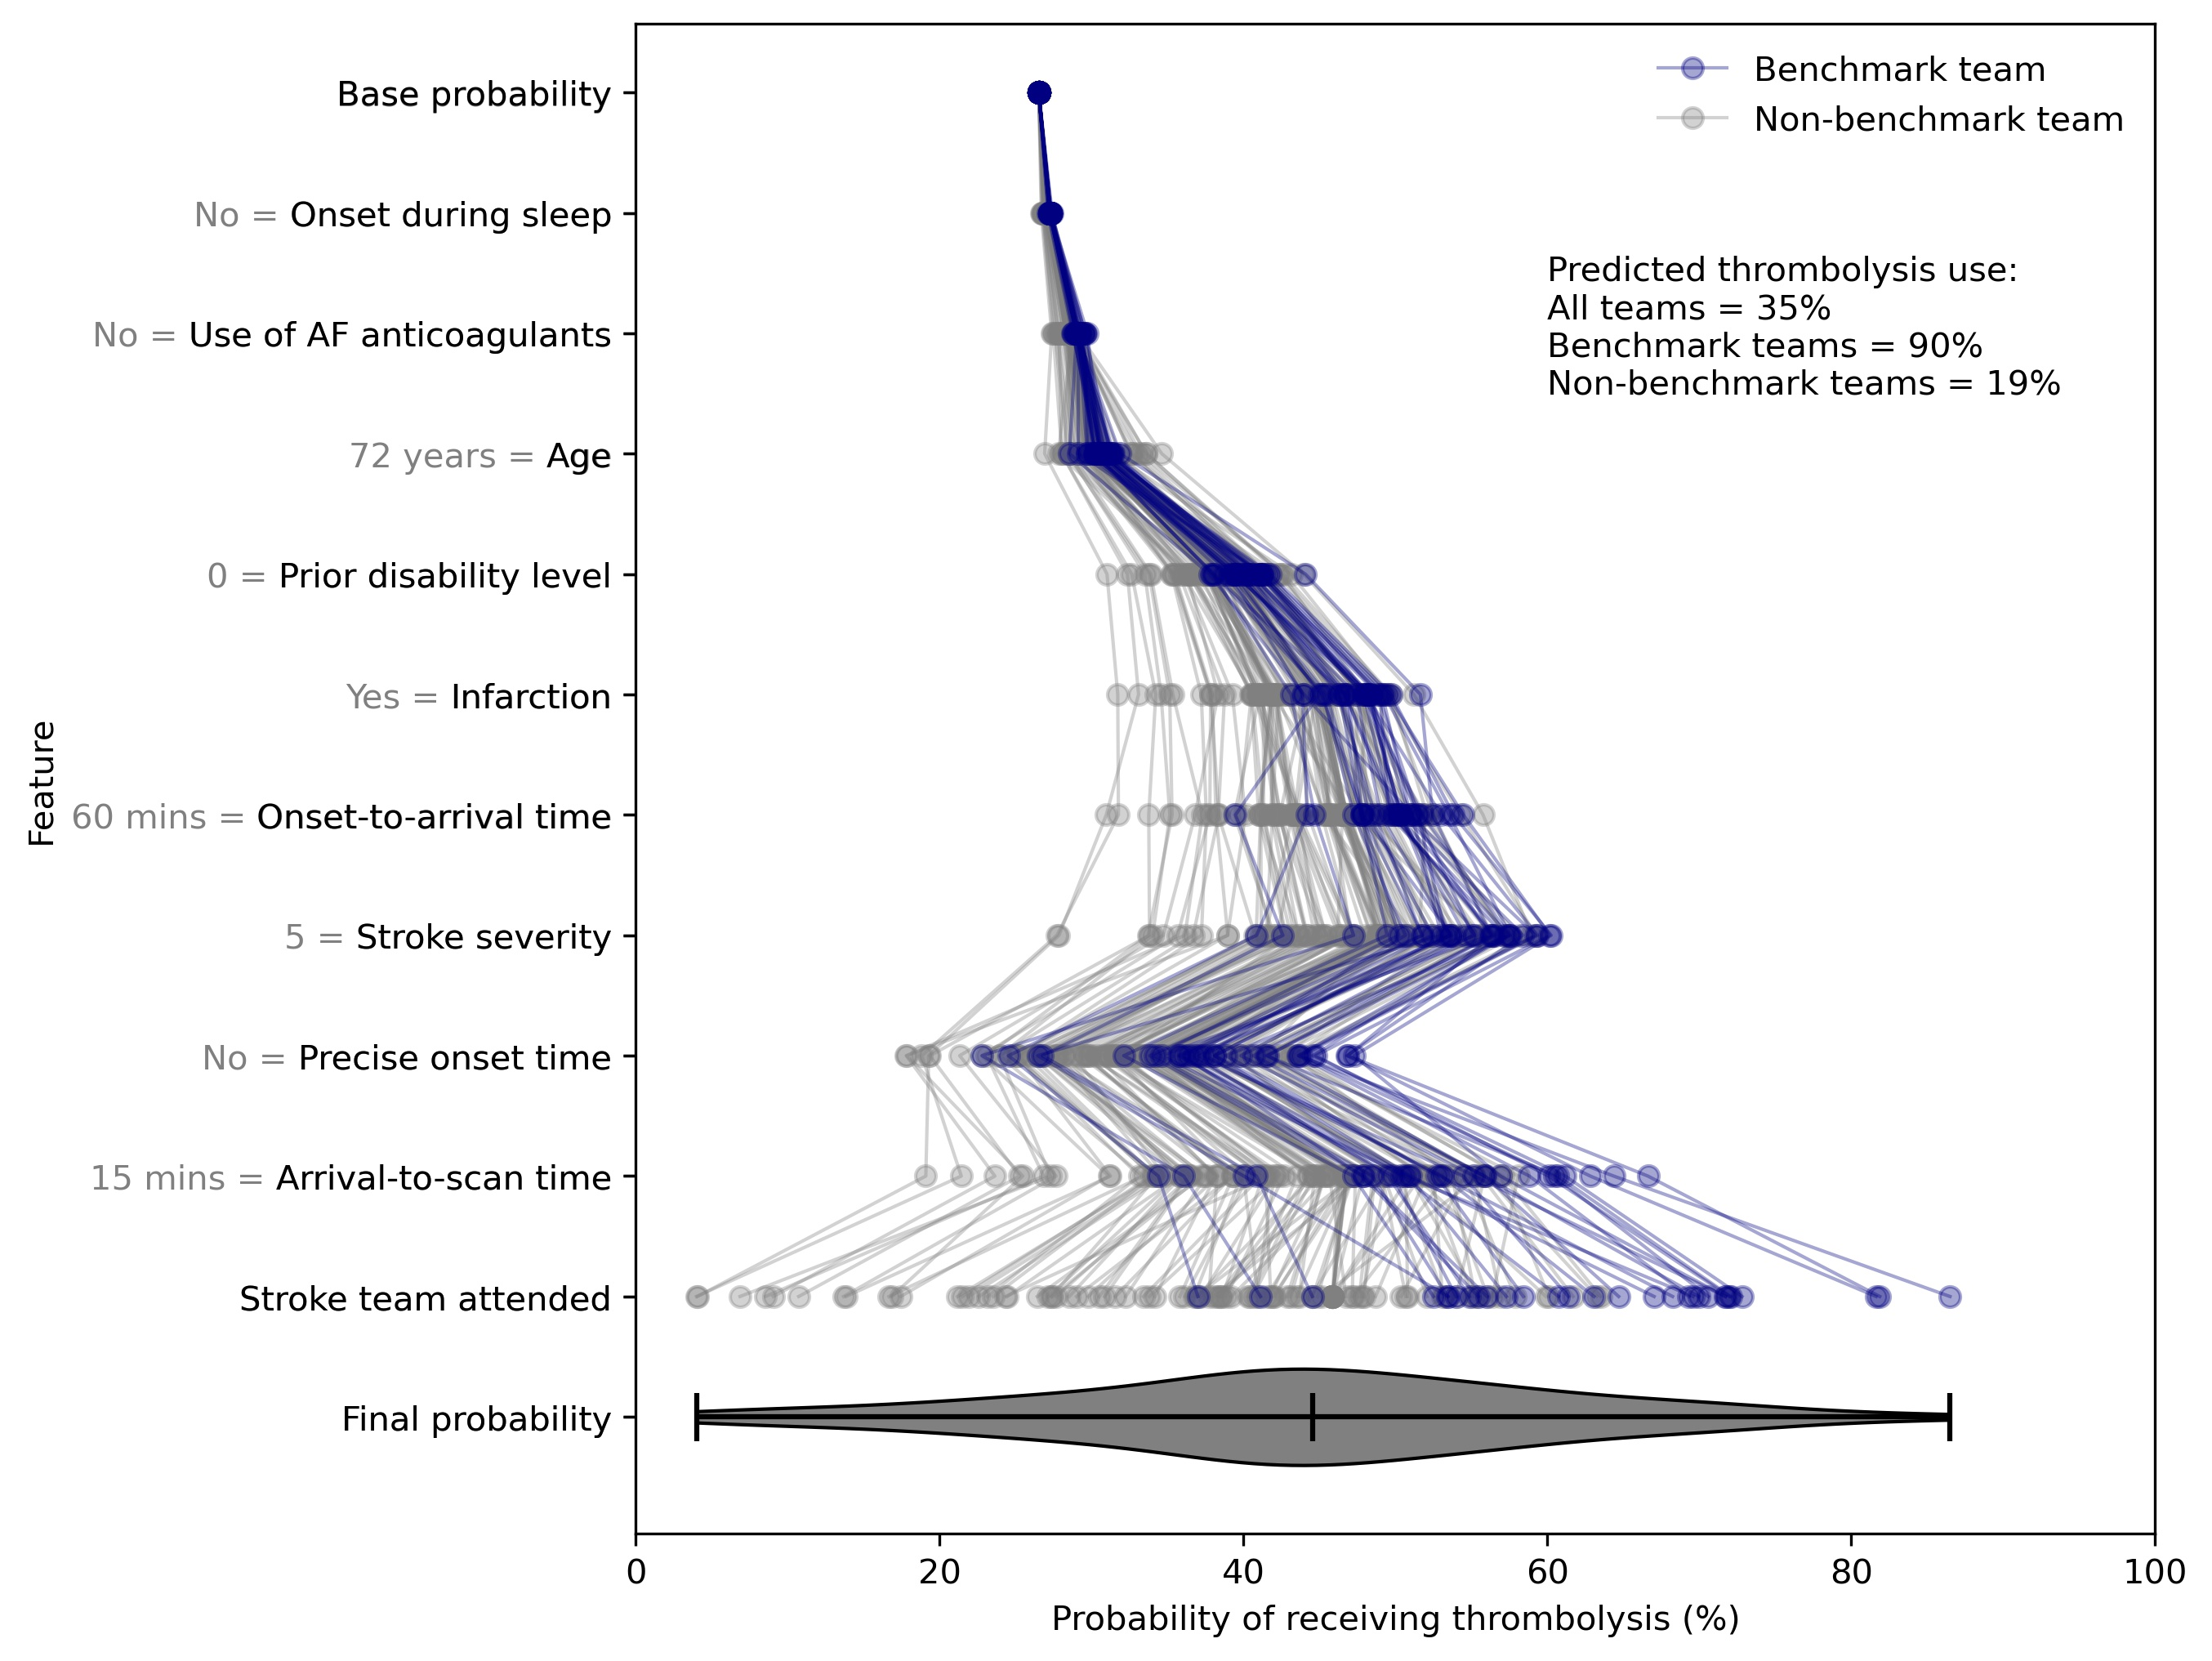
\includegraphics[width=0.7\textwidth]{./images/21_shap_waterfall_with_violin_contentious.jpg}
    \end{center}

\footnotesize The patient starts with the same base probability, then each hospital reacts differently when presented with each of the patients characteristics and nudges the probability to a different level.

\end{frame}


\begin{frame}
\frametitle{Summary}

\begin{itemize}
    \setlength{\itemsep}{2.5mm}
    \item The XGBoost/SHAP model revealed that the odds of receiving thrombolysis:    
    \begin{itemize}
        \vspace{2mm}
        \setlength{\itemsep}{2.5mm}
        \item Reduced 20+ fold with increasing arrival-to-scan time
        \item Varied 30 fold depending on stroke severity
        \item Reduced 3 fold with imprecise onset time (and another 4-fold if onset was during sleep)
        \item Fell 5 fold with increasing pre-stroke disability
        \item Varied 15 fold between hospitals.
        \item Fell 5 fold if the patient was taking anticoagulant medication
        \item Fell 3 fold between two and four hours arrival-to-onset time
    \end{itemize}

\item The hospital identification (hospital SHAP value) explained 58\% of the variance in between-hospital thrombolysis use. 
\end{itemize}

\end{frame}

\begin{frame}
\frametitle{Jupyter book of all code and results}

\scriptsize
\url{https://samuel-book.github.io/samuel_shap_paper_1/introduction/intro.html}

\vspace{3mm}



\begin{center}

\includegraphics[width=0.45\textwidth]{./images/qr_shap_1_jupyter_book}
\end{center}


\end{frame}

%%%%%%%%%%%%%%%%%%%%%%%%%%%%%%%%%%%%%%%%%%%%%%%%%%%%%%%%%%%%%%%

\end{document}




